\section{Introducción}

% Considere que las referencias están en formato \textit{Bibitems} y se incluyen al final de este archivo.

Este es un ejemplo de como se deben insertar referencia en el documento~\cite{conagua-2011}. Considere que las referencias están en formato \textit{Bibitems} y se incluyen al final de este archivo~\cite{conagua-2011,undesa2008}.


% Texto dummy para rellenar el documento
\blindtext[2]

 % ejemplo de figura
\begin{figure}[htb]
    \centering
    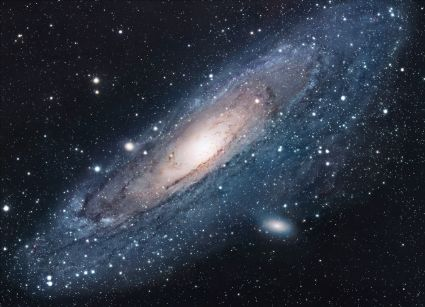
\includegraphics[width=3.5in]{images/universe}
    \caption{Pie de texto en la figura.}
    \label{fig:universe}
\end{figure}

\blindtext[3]